\chapter{Testing e valutazione dei risultati}
\label{capitolo7}
\thispagestyle{empty}
In questo capitolo vedremo le diverse fasi di testing e analizzeremo gli effetti del nuovo software sulle tempistiche di integrazione e in termini di aumento del numero di collegamenti effettuati con la centrale operativa.
\section{Testing}
La fase di testing del software si può dividere in tre sotto-fasi che analizzeremo in maniera distinta tuttavia facciamo una breve premessa riguardo all'architettura utilizzata per il testing.
\subsection{L'architettura del testing}
Per testare il nuovo software sono state create una serie di macchine virtuali per replicare esattamente l'architettura di produzione; inoltre, per quanto riguarda i ricevitori, la modularità del nuovo software ha permesso di escludere i ricevitori non necessari o quelli ampiamente testati. Per testare la ricezione degli allarmi si avevano a disposizione fisicamente le centrali di allarme a banco.\\
Ogni software è stato pensato per essere analizzato a diverso livello, infatti, ogni software sfrutta il demone \emph{syslog} dell'ambiente linux per scrivere diversi file di log, inoltre lo stesso demone permette di impostare il livello di log in base a sette livelli i quali servono a distinguere i messaggi più gravi da quelli necessari solo all'analisi del software. Inoltre tutto il software è stato pensato per un ulteriore divisione dei messaggi, infatti è possibile impostare il software in modo da decidere se è necessario scrivere sul file di log anche le query eseguite sul database o effettuare il log di un singolo ricevitore o telegestore.
\subsection{La prima fase di testing}
In una prima fase di testing il nuovo software viene testato singolarmente in modo da escludere l'interazione con il resto del sistema. Il nuovo software viene introdotto nell'ambiente di test, e gli unici processi eseguiti sono quello del database sul quale il nuovo software si appoggia ed il software stesso. Prendendo in considerazione, ad esempio, il software di ricezione degli allarmi e volendo testare un nuovo ricevitore, si disabilitano tutti gli altri ricevitori in modo che gli unici thread in esecuzione siano quello del controllore e quello del nuovo ricevitore da testare. A questo punto tramite una centrale d'allarme a banco si effettuano dei test controllati, in primo luogo si verifica lo stato della connessione e la corretta comunicazione dei messaggi tramite il file di log del ricevitore. Nel caso in cui la comunicazione non avvenisse in modo corretto si utilizzano diversi strumenti per l'analisi dei messaggi tra i quali \emph{Wireshark}\cite{wireshark}.\\
In caso di successo, invece, si passava a testare la validità del software ovvero, ad analizzare se gli eventi ricevuti vengono convertiti in un allarme vero e proprio dal software; per fare ciò si testano un sottoinsieme di eventi normalmente generati da una centrale d'allarme, in particolare si testano:
\begin{itemize}
	\item inserimento e disinserimento di una partizione;
	\item esclusione od inclusione di una zona;
	\item manomissione della centrale;
	\item manomissione di un sensore.
	\item Allarme di una zona
\end{itemize}
In particolare per le ultime due tipologie di segnalazioni ci serviamo di un hardware che sfrutta la configurazione dei sensori a \emph{doppio bilanciamento} in particolare in \fname{fig:sensdoppio} vediamo lo schema elettrico del collegamento di un sensore collegato in doppio bilanciamento, mentre in \fname{fig:schemadoppio} vediamo lo schema del nostro hardware, intervenendo sul contatto di \emph{tamper} si testa la manomissione del sensore mentre intervenendo sul \emph{contatto d'allarme} si testa l'allarme della zona.
\begin{figure}
	\centering
	\subfigure[]{
		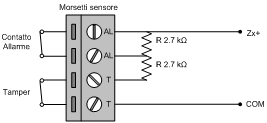
\includegraphics[width=0.4\linewidth]{pictures/doppiobilanciamento.png}\label{fig:sensdoppio}
	}
	\subfigure[]{
		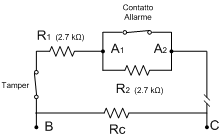
\includegraphics[width=0.4\linewidth]{pictures/b24-schema2.png}\label{fig:schemadoppio}
	}
	\caption{Configurazione di un sensore in doppio bilanciamento e schema dell'hardware di test}
\end{figure}
Per quanto riguarda il software di telegestione la fase di testing procede nello stesso modo fino a questo punto, ovvero verifica della connessione e del corretto scambio di informazioni; la validazione tuttavia consiste nel verificare il corretto invio dei comandi alla centrale e in secondo luogo la corretta traduzione degli elementi della centrale. In particolare i comandi che vengono controllati sono:
\begin{itemize}
	\item inserimento e disinserimento di una partizione;
	\item inclusione o esclusione di una zona;
\end{itemize}
Gli stati monitorati sono:
\begin{itemize}
	\item per la centrale: lo stato dell'alimentazione elettrica, lo stato della batteria e lo stato del contatto di manomissione;
	\item per le partizioni: lo stato di inserimento o di disinserimento o di inserimento parziale;
	\item per le zone: lo stato di allarme, lo stato di riposo o lo stato di esclusione
\end{itemize}
Una volta verificato il corretto funzionamento del software si passa a testare l'affidabilità mantenendo in esecuzione il software per almeno una giornata e generando periodicamente un evento o inviando un comando.\\
Nel caso in cui anche questa fase di test sia superata si testa il sistema nel suo insieme attivando anche il resto dei moduli non necessari anche nell'ambiente di test. Se anche in questo caso non si verificano errori il sistema è ritenuto abbastanza stabile e affidabile da poter essere rilasciato in produzione.
\subsection{$\alpha$-testing}
Dopo che il software ha superato la prima fase di testing si passa alla seconda nella quale la nuova versione del programma viene rilasciata sulle macchine di produzione. Dopo aver caricato l'eseguibile si programmano gli script di controllo per monitorare e, in caso di malfunzionamento, riavviare il software. In caso di crash inoltre questi sistemi di controllo inviano una mail per tenere traccia del momento esatto del riavvio. Tramite questo meccanismo è possibile risalire nel file di log all'evento che ha scatenato il blocco del sistema senza mantenere monitorato il file.\\
In questa fase il nuovo software viene avviato nell'architettura di produzione e lasciato in esecuzione, ad esso vengono collegate diverse centrali le quali tuttavia sono sempre centrali di prova collegate all'interno dell'azienda per poter intervenire in modo rapido e completo sulla centrale e cercare un riscontro dell'evento che ha eventualmente generato il crash del sistema. In questo modo è possibile testare il sistema con un carico di eventi sempre basso ma che comunque impegna il sistema anche in modo concorrente permettendo così di individuare eventuali problemi di concorrenza tra i thread.
Per quanto riguarda il \texttt{Telegestore}, invece, permette di studiare il comportamento con sensori situati in un ambiente reale anche se controllato.\\
Essendo questo test effettuato in ambiente di produzione gli eventi ricevuti dalle centrali collegate a questo ricevitore verrebbero mostrati agli operatori, per evitare ciò è possibile selezionare un parametro nella configurazione della centrale nel software E-Pro che permette di registrare gli allarmi sul database ma di renderli passanti ovvero di non mostrarli agli operatori.\\
Lo scopo principale di questo tipo di testing è quello di individuare problemi di concorrenza e di verificare in modo più approfondito la stabilità del sistema il quale è un requisito fondamentale per questi software.
\subsection{$\beta$-testing}
Alla fine della fase di $ \alpha$-test il nuovo software è già in produzione e risulta abbastanza stabile, tuttavia il numero di segnalazioni o di gestioni è molto ridotto in quanto il numero di centrali collegate è inferiore a dieci mentre a pieno ritmo i collegamenti possibili sono anche dell'ordine delle migliaia di centrali.\\
Per progredire nel testing del software si passa alla fase di $ \beta$-test nella quale vengono collegate al nuovo ricevitore diverse centrali selezionate tra quelle già installate dai clienti in modo da avere un numero più elevato di segnalazioni anche contemporanee provenienti almeno da un centinaio di centrali.\\
Questa fase è un vero e proprio stress test del nuovo software il quale deve essere in grado di sopportare il carico delle segnalazioni o delle telegestioni.\\
In questo caso le segnalazioni vengo gestite dagli operatori e siamo quasi nella situazione di normale funzionamento, tuttavia rispetto alla situazione standard le centrali selezionate come $ \beta$-tester dispongono anche di un sistema di backup che è in grado di inviare le segnalazioni di allarme anche tramite un altro vettore e quindi destinate ad un ricevitore diverso da quello testato.\\
Durante questa fase si individuano eventuali problemi di concorrenza su larga scala, eventuale sottodimensionamento delle risorse del ricevitore ed eventuali errori di traduzione degli allarmi.
\section{Valutazione dei risultati}
Analizziamo ora in termini numerici quali sono stati i miglioramenti che il nostro lavoro ha portato all'interno dell'azienda. In particolare possiamo analizzare i miglioramenti in termini di velocità di integrazione e\emph{ “time to market”}, analizzando la riduzione delle tempistiche di gestione delle segnalazioni ed il carico del sistema, infine possiamo fare riferimento anche all'aumento del numero di collegamenti alla centrale.\\
In particolare per quanto riguarda la fase di integrazione possiamo distinguere due tempistiche, la prima che ha riguardato la fase di progettazione del software che ha richiesto all'incirca quattro mesi ma che si è svolta un'unica volta e la seconda tempistica che si ha ogni qualvolta che si deve integrare un nuovo protocollo di ricezione che è nell'ordine di due settimane dal momento della ricezione del protocollo al termine della prima fase di testing, in base alla complessità del protocollo. Prima del nostro intervento questa fase poteva richiedere anche alcuni mesi a causa della complessità della logica del software precedentemente creato che non permetteva l'inserimento di un nuovo ricevitore senza interferire con il resto del codice.\\
Per quanto riguarda la riduzione dei tempi di gestione è dovuta a due fattori principali, la riduzione dei tempi di trasmissione degli eventi e la riduzione dei tempi di gestione degli operatori tramite l'utilizzo della telegestione. Per quanto riguarda la riduzione dei tempi di trasmissione si è passati da un tempo di trasmissione dell'ordine dei \emph{20s} in caso di comunicazione su PSTN ad un tempo inferiore ai \emph{2s} per trasmissioni tramite TCP/IP inoltre, il ricevitore PSTN poteva ricevere fino a dieci comunicazioni simultanee, con un ricevitore software il numero di connessioni simultanee è stato limitato a 250 per singolo ricevitore. Per quanto riguarda invece, la vera e propria gestione dell'evento da parte degli operatori, si è notato un riduzione del 20\% dei tempi di gestione soprattutto grazie alla telegestione che permette di eseguire le operazioni più comuni sulle centrali direttamente dal software E-Pro senza dover cambiare postazione per accedere al software di telegestione specifico per il tipo di centrale.\\
Una diretta conseguenza della facilità di integrazione di nuovi ricevitori e della telegestione di nuove centrali è l'aumento del numero di collegamenti con la centrale operativa e il conseguente aumento del numero di clienti; questo aumento è quantificabile con il 10\% in più dei clienti gestiti.